\newpage
\def\thoigian{90}%--Thời gian
\de{Đề số 3}{Chương V. Vectơ}

\begin{center}
	\textbf{PHẦN 1 - CÂU TRẮC NGHIỆM BỐN PHƯƠNG ÁN}
\end{center}
\Opensolutionfile{ans}[ans/ans-TN-ONTAPCHUONG-DE4]
%Câu 1

\begin{ex}%[0H5N1-2]%[Dự án D - đợt 4 NH24-25-Đoàn Minh Tâm]
	\immini{Cho hình lục giác đều $ABCDEF$ có tâm là $O$ như hình vẽ. Có bao nhiêu vectơ cùng hướng với $\overrightarrow{AB}$?
		\choice
		{$5$}
		{\True $4$}
		{$3$}
		{$7$}
	}
	{\begin{tikzpicture}[>=stealth,line join=round,line cap=round,font=\footnotesize,scale=0.3]
			\path (0,0) coordinate (O)
			($(O)+({5*cos(120)},{5*sin(120)})$) coordinate (A)
			($(O)+({5*cos(60)},{5*sin(60)})$) coordinate (B)
			($(O)+({5*cos(0)},{5*sin(0)})$) coordinate (C)
			($(O)+({5*cos(-60)},{5*sin(-60)})$) coordinate (D)
			($(O)+({5*cos(-120)},{5*sin(-120)})$) coordinate (E)
			($(O)+({5*cos(-180)},{5*sin(-180)})$) coordinate (F)
			;
			\draw (A)--(B)--(C)--(D)--(E)--(F)--(A) (A)--(D) (B)--(E) (C)--(F);
			\foreach \p / \r in {A/135,B/45,C/0,D/-45,E/-135,F/180,O/90}
			\fill (\p) circle (1.2pt) node[shift={(\r:4mm)}]{$\p$};
	\end{tikzpicture}}
	\loigiai{
		Các vectơ cùng hướng với $\overrightarrow{AB}$ là $\overrightarrow{FO}$, $\overrightarrow{FC}$, $\overrightarrow{OC}$, $\overrightarrow{ED}$.}
\end{ex}

\begin{ex}%[0H5N1-1]%[Dự án D - đợt 4 NH24-25-Đoàn Minh Tâm]
	Nếu $\overrightarrow{AB}=\overrightarrow{AC}$ thì khẳng định nào sau đây \textbf{đúng}?
	\choice
	{Tam giác $ABC$ là tam giác cân}
	{Điểm $A$ là trung điểm đoạn $BC$}
	{\True Điểm $B$ trùng với điểm $C$}
	{Tam giác $ABC$ là tam giác đều}
	\loigiai{
		Nếu $\overrightarrow{AB}=\overrightarrow{AC}$ thì điểm $B$ trùng với điểm $C$.
	}
\end{ex}

\begin{ex}%[0H5N1-5]%[Dự án D - đợt 4 NH24-25-Đoàn Minh Tâm]
	Cho hình vuông $ABCD$ có cạnh bằng $2a$. Tính độ dài của vectơ $\overrightarrow{BD}$.
	\choice
	{\True $2a\sqrt{2}$}
	{$a\sqrt{2}$}
	{$8a$}
	{$2a$}
	\loigiai{
		\immini{Ta có theo quy tắc hình bình hành thì  $$\left|\overrightarrow{BD}\right|=BD=\sqrt{AB^2+AD^2}=\sqrt{4a^2+4a^2}=2a\sqrt{2}.$$}
		{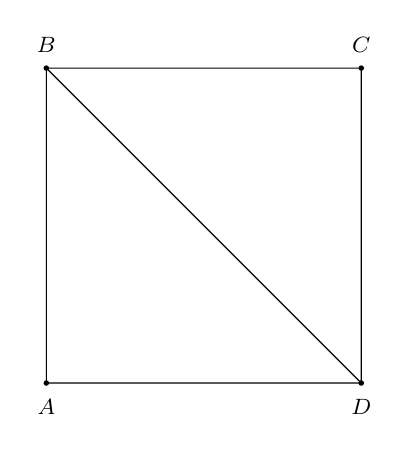
\begin{tikzpicture}[scale=1, font=\footnotesize, line join=round, line cap=round,>=stealth]
				\path
				(0,0) coordinate (A)
				(4,4) coordinate (C)
				(0,4) coordinate (B)
				(4,0) coordinate (D)
				;
				\draw  (A)--(B)--(C)--(D)--(A) (B)--(D);
				\foreach \x/\g in {A/-90,B/90,C/90,D/-90}
				\fill[black] (\x) circle (1pt)+(\g:3mm) node {$\x$};
		\end{tikzpicture}}
	}
\end{ex}
%Câu 4
\begin{ex}%[0H5N2-1]%[Dự án D - đợt 4 NH24-25-Đoàn Minh Tâm]
	Cho tam giác $ABC$ có trọng tâm $G$ tổng ba vectơ $\overrightarrow{GA}+\overrightarrow{GB}+\overrightarrow{GC}$ bằng
	\choice
	{$\overrightarrow{CB}$}
	{$\overrightarrow{AC}$}
	{$\overrightarrow{BC}$}
	{\True $\overrightarrow{0}$}
	\loigiai{
		Với $G$ là trọng tâm tam giác $ABC$ ta có $\overrightarrow{GA}+\overrightarrow{GB}+\overrightarrow{GC}=\overrightarrow{0}$.
	}
\end{ex}


\begin{ex}%[0H5H2-2]%[Dự án D - đợt 4 NH24-25-Đoàn Minh Tâm]
	Gọi $O$ là tâm hình bình hành $ABCD$; hai điểm $E$, $F$ lần lượt là trung điểm $AB$, $BC$. Đẳng thức nào sau đây \textbf{sai}?
	\choice
	{$\overrightarrow{DO}=\overrightarrow{EB}-\overrightarrow{EO}$}
	{$\overrightarrow{OC}=\overrightarrow{EB}+\overrightarrow{EO}$}
	{\True $\overrightarrow{BE}+\overrightarrow{BF}-\overrightarrow{DO}=\vec{0}$}
	{$\overrightarrow{OA}+\overrightarrow{OC}+\overrightarrow{OD}+\overrightarrow{OE}+\overrightarrow{OF}=\vec{0}$}
	\loigiai{
		\immini{
			Ta có $OF$, $OE$ lần lượt là đường trung bình của tam giác $BCD$ và $ABC$.\\
			Suy ra $BEOF$ là hình bình hành.\\
			Khi đó $\overrightarrow{BE}+\overrightarrow{BF}=\overrightarrow{BO}$.\\
			Suy ra $\overrightarrow{BE}+\overrightarrow{BF}-\overrightarrow{DO}=\overrightarrow{BO}-\overrightarrow{DO}=\overrightarrow{OD}-\overrightarrow{OB}=\overrightarrow{BD}$.
		}{\begin{tikzpicture}[line join=round,line cap=round,>=stealth,scale=1,font=\footnotesize]
				\foreach \x/\y/\n in {0/0/A,3/0/D,-1/-2/B} \coordinate (\n) at (\x,\y);
				\coordinate (C) at ($(B)+(D)-(A)$);
				\coordinate (E) at ($(A)!1/2!(B)$);
				\coordinate (F) at ($(B)!1/2!(C)$);
				\coordinate (O) at ($(A)!1/2!(C)$);
				\draw (A)--(B)--(C)--(D)--(A)--(C) (B)--(D) (O)--(E)--(F)--(O);
				\foreach \t/\g in {A/90,B/-135,C/-45,D/45,E/180,F/-90,O/90}{
					\draw[fill=black] (\t) circle (1pt) node[shift={(\g:8pt)}]{$ \t $};
				}
		\end{tikzpicture}}
	}
\end{ex}
\begin{ex}%[0H5H2-3]%[Dự án D - đợt 4 NH24-25-Đoàn Minh Tâm]
	Cho tam giác $ABC$. Nếu điểm $M$ thỏa mãn $\overrightarrow{MA}-\overrightarrow{MB}-\overrightarrow{MC}=\overrightarrow{0}$ thì khi đó
	\choice
	{$M$ là trung điểm $BC$}
	{$M$ là trung điểm $AB$}
	{$ABMC$ là hình bình hành}
	{\True $ABCM$ là hình bình hành}
	\loigiai{
		\immini{Ta có $\overrightarrow{MA}-\overrightarrow{MB}-\overrightarrow{MC}=\overrightarrow{0}\Leftrightarrow\overrightarrow{BA}=\overrightarrow{MC}$.\\
			Suy ra tứ giác $ABCM$ là hình bình hành.}
		{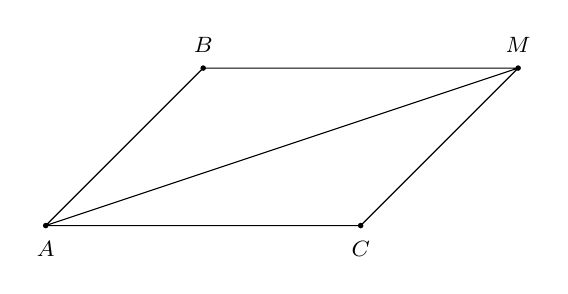
\begin{tikzpicture}[scale=1, font=\footnotesize, line join=round, line cap=round,>=stealth]
				\path
				(0,0) coordinate (A)
				(6,2) coordinate (M)
				(2,2) coordinate (B)
				(4,0) coordinate (C)
				;
				\draw  (A)--(B)--(M)--(C)--(A)--(M);
				\foreach \x/\g in {A/-90,B/90,M/90,C/-90}
				\fill[black] (\x) circle (1pt)+(\g:3mm) node {$\x$};
		\end{tikzpicture}}
	}
\end{ex}
%Câu 7

\begin{ex}%[0H5N3-1]%[Dự án D - đợt 4 NH24-25-Đoàn Minh Tâm]
	Trên đường thẳng $ MN$ lấy điểm $P$ sao cho $\overrightarrow{M N}=-3 \overrightarrow{M P}$. Điểm $P$ được xác định đúng trong hình vẽ nào sau đây
	\begin{center}
		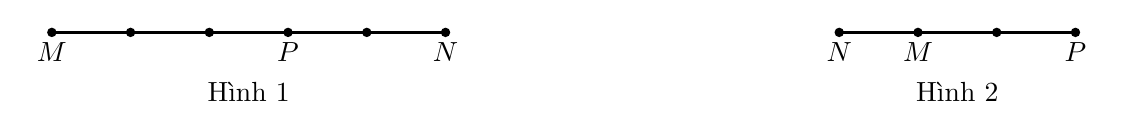
\begin{tikzpicture}[line join=round, line cap=round,>=stealth,thick]
			\fill (0,0) circle (.06) node[below ]{$M$};
			\foreach \x in {1,2,3,4,5} \fill (\x,0) circle (.06);
			\draw (3,0) node[below]{$ P $};
			\draw (5,0) node[below]{$ N $};
			\draw (0,0)--(5,0);
			\draw (2.5,-.5) node[below]{Hình $1$};
			\fill (10,0) circle (.06) node[below ]{$N$};
			\foreach \x in {11,12,13} \fill (\x,0) circle (.06);
			\draw (11,0) node[below]{$ M $};
			\draw (13,0) node[below]{$ P $};
			\draw (10,0)--(13,0);
			\draw (11.5,-.5) node[below]{Hình $2$};
		\end{tikzpicture}
	\end{center}
	\begin{center}
		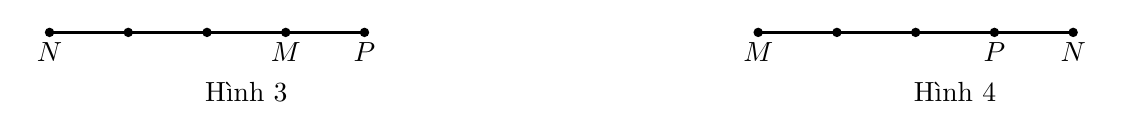
\begin{tikzpicture}[line join=round, line cap=round,>=stealth,thick]
			\fill (0,0) circle (.06) node[below ]{$N$};
			\foreach \x in {1,2,3,4} \fill (\x,0) circle (.06);
			\draw (3,0) node[below]{$ M $};
			\draw (4,0) node[below]{$ P $};
			\draw (0,0)--(4,0);
			\draw (2.5,-.5) node[below]{Hình $3$};
			\fill (9,0) circle (.06) node[below ]{$M$};
			\foreach \x in {10,11,12,13} \fill (\x,0) circle (.06);
			\draw (12,0) node[below]{$ P$};
			\draw (13,0) node[below]{$ N $};
			\draw (9,0)--(13,0);
			\draw (11.5,-.5) node[below]{Hình $4$};
		\end{tikzpicture}
	\end{center}
	\choice
	{Hình $4$}
	{Hình $1$}
	{Hình $2$}
	{\True Hình $3$}
	\loigiai{
		Ở Hình $3$ ta thấy $MN=3MP$ và $\overrightarrow{MN}$, $\overrightarrow{MP}$ là hai vectơ đối nhau. \\
		Do đó $\overrightarrow{M N}=-3 \overrightarrow{M P}$.
	}
\end{ex}
\begin{ex}%[0H5N3-2]%[Dự án D - đợt 4 NH24-25-Đoàn Minh Tâm]
	Cho tam giác $ABC$ có $I$ là trung điểm $AB$. Mệnh đề nào sau đây đúng?
	\choice
	{$\overrightarrow{CA}-\overrightarrow{CB}=2\overrightarrow{CI}$}
	{$\overrightarrow{CA}+\overrightarrow{CI}=2\overrightarrow{CB}$}
	{\True $\overrightarrow{CA}+\overrightarrow{CB}=2\overrightarrow{CI}$}
	{$\overrightarrow{CI}+\overrightarrow{CB}=2\overrightarrow{CA}$}
	\loigiai{
		Với $I$ là trung điểm $AB$ thì $\overrightarrow{CA}+\overrightarrow{CB}=2\overrightarrow{CI}$.
	}
\end{ex}
\begin{ex}%[0H5H3-6]%[Dự án D - đợt 4 NH24-25-Đoàn Minh Tâm]
	Cho hình vuông $ABCD$ cạnh $a$. Tính $\left|\overrightarrow{AB}+\overrightarrow{AC}+\overrightarrow{AD}\right|$.
	\choice
	{$\left(2+\sqrt{2}\right)a$}
	{$3a$}
	{\True $2\sqrt{2}a$}
	{$a\sqrt{2}$}
	\loigiai
	{\immini
		{Ta có
			$$\left|\overrightarrow{AB} + \overrightarrow{AC} + \overrightarrow{AD}\right| = \left|\overrightarrow{AC} + \overrightarrow{AC}\right| = 2AC = 2a\sqrt{2}.$$
		}
		{\begin{tikzpicture}[scale=1, font=\footnotesize,line join=round, line cap=round, >=stealth]
				\def\a{3}
				\path (0,0) coordinate (B)
				(\a,0) coordinate (C)
				++(0,\a) coordinate (D)
				++(-\a,0) coordinate (A);
				\draw (A)--(B)--(C)--(D)--cycle;
				\foreach \diem/\pos in {B/-90, C/-90, A/90, D/90} \fill (\diem) node[shift={(\pos:0.3)}] {$\diem$} circle(1pt);
	\end{tikzpicture}}}
\end{ex}
%Câu 10
\begin{ex}%[0H5H4-1]%[Dự án D - đợt 4 NH24-25-Đoàn Minh Tâm]
	Cho tam giác $ABC$ vuông cân tại $A$. Góc giữa hai vectơ $\overrightarrow{BA}$ và $\overrightarrow{BC}$ bằng
	\choice
	{$180^\circ$}
	{$0^\circ$}
	{$30^\circ$}
	{\True $45^\circ$}
	\loigiai{
		Vì $\triangle{ABC}$ vuông cân tại $A$ nên suy ra $\widehat{ABC}=45^\circ$.
	}
\end{ex}

\begin{ex}%[0H5H4-1]%[Dự án D - đợt 4 NH24-25-Đoàn Minh Tâm]
	Cho hai vectơ $\overrightarrow{a}$ và $\overrightarrow{b}$ khác $\overrightarrow{0}$, $\alpha$ là góc tạo bởi hai vectơ $\overrightarrow{a}$ và $\overrightarrow{b}$. Nếu $\overrightarrow{a}\cdot\overrightarrow{b}=-\left|\overrightarrow{a}\right|\cdot\left|\overrightarrow{b}\right|$ thì $\alpha$ nhận giá trị nào trong các giá trị dưới đây?
	\choice
	{$0^\circ$}
	{$45^\circ$}
	{\True $180^\circ$}
	{$90^\circ$}
	\loigiai{
		Ta có $\cos\alpha=\dfrac{\overrightarrow{a}\cdot\overrightarrow{b}}{\left|\overrightarrow{a}\right|\cdot\left|\overrightarrow{b}\right|}=-1\Rightarrow\alpha=180^0$.
	}
\end{ex}


\begin{ex}%[0H5H4-1]%[Dự án D - đợt 4 NH24-25-Đoàn Minh Tâm]
	Cho tam giác $ABC$ đều cạnh bằng $4$. Tính tích vô hướng $\overrightarrow{AB}\cdot\overrightarrow{BC}$.
	\choice
	{$8$}
	{$-8\sqrt{3}$}
	{$8\sqrt{3}$}
	{\True $-8$}
	\loigiai{
		Ta có $\overrightarrow{AB}\cdot\overrightarrow{BC}=AB\cdot BC\cdot\cos(\overrightarrow{AB},\overrightarrow{BC})=4\cdot4\cdot\cos120^\circ=-8$.
	}
\end{ex}

\Closesolutionfile{ans}
%\begin{center}
%	\textbf{ĐÁP ÁN}
%	\inputansbox{10}{ans/ans}
%\end{center}



\begin{center}
	\textbf{PHẦN 2 - CÂU TRẮC NGHIỆM ĐÚNG SAI}
\end{center}

\Opensolutionfile{ans}[ans/answer-DS-ONTAPCHUONG-DE4]
\setcounter{ex}{0}
\begin{ex}%[0H5V2-2]%[Dự án D - đợt 4 NH24-25-Đoàn Minh Tâm]
	Cho hình bình hành $ABCD$ tâm $O$.
	\choiceTF
	{$\overrightarrow{OA}-\overrightarrow{OB}+\overrightarrow{DC}=\overrightarrow{CB}$}
	{\True $\overrightarrow{BA}+\overrightarrow{AB}=\vec{0}$}
	{\True $\overrightarrow{OA}+\overrightarrow{AC}=\overrightarrow{OC}$}
	{\True $\overrightarrow{OB}+\overrightarrow{OA}-\overrightarrow{CA}=\overrightarrow{DC}$}
	\loigiai{
		\begin{itemchoice}
			\itemch Vì $\overrightarrow{OA}-\overrightarrow{OB}+\overrightarrow{DC}=\overrightarrow{OA}+\overrightarrow{BO}+\overrightarrow{DC}=\overrightarrow{BO}+\overrightarrow{OA}+\overrightarrow{AB}=\overrightarrow{BA}+\overrightarrow{AB}=\overrightarrow{0}$.
			\itemch Vì $\overrightarrow{BA}+\overrightarrow{AB}=\overrightarrow{BB}=\vec{0}$.
			\itemch Vì $\overrightarrow{OA}+\overrightarrow{AC}=\overrightarrow{OC}$ (quy tắc ba điểm).
			\itemch Vì $\overrightarrow{OB}+\overrightarrow{OA}-\overrightarrow{CA}=\overrightarrow{OB}+\overrightarrow{OA}+\overrightarrow{AC}=\overrightarrow{OB}+\overrightarrow{OC}=\overrightarrow{DO}+\overrightarrow{OC}=\overrightarrow{DC}$.
		\end{itemchoice}}
\end{ex}
\begin{ex}%[0H5H2-4]%[Dự án D - đợt 4 NH24-25-Đoàn Minh Tâm]
	Cho hình vuông $ABCD$ cạnh $a$.
	\choiceTF
	{$|\overrightarrow{AB}+\overrightarrow{AD}|=a\sqrt{2}$}
	{\True Gọi $M$, $N$ lần lượt là trung điểm của đoạn thẳng $BC$ và $AD$. Khi đó $\left|\overrightarrow{NC}+\overrightarrow{MC}\right|=a\sqrt{2}$}
	{\True  Độ dài của $\overrightarrow{u}=4\overrightarrow{MA}-3\overrightarrow{MB}+\overrightarrow{MC}-2\overrightarrow{MD}$ là $a\sqrt{5}$}
	{Với $O$ là giao điểm của $AC$ và $BD$. Khi đó $|\overrightarrow{OA}+\overrightarrow{OB}|=a\sqrt{2}$}
	\loigiai{
		\begin{center}
			\begin{tikzpicture}[scale=1, font=\footnotesize, line join=round, line cap=round,>=stealth]
				\path
				(0,0) coordinate(A)
				(2,2) coordinate(C)
				(0,2) coordinate(B)
				(2,0) coordinate(D)
				($(A)!.5!(D)$)coordinate (N)
				($(B)!.5!(C)$)coordinate (M)
				(intersection of A--C and B--D)coordinate(O)
				($(O)!3!(A)$)coordinate (A')
				;
				\draw(A)--(B)--(C)--(D)--(A)--(M)(N)--(C)(A)--(C)(B)--(D) (A)--(A')--(B);
				\foreach \x/\g in{A/-90,B/90,C/90,D/-90,M/90,N/-90,O/-90,A'/180}
				\fill[black](\x) circle(1pt)+(\g:3mm) node{$\x$};
			\end{tikzpicture}
		\end{center}
		\begin{itemchoice}
			\itemch Ta có $|\overrightarrow{AB}+\overrightarrow{AD}|=|\overrightarrow{AC}|=a\sqrt{2}$.
			\itemch Ta có $\left|\overrightarrow{NC}+\overrightarrow{MC}\right|=\left|\overrightarrow{AM}+\overrightarrow{MC}\right|=\left|\overrightarrow{AC}\right|=AC=a\sqrt{2}$.
			\itemch Ta có
			\allowdisplaybreaks
			\begin{eqnarray*}
				\overrightarrow{u} &=&4\overrightarrow{MA}-3\overrightarrow{MB}+\overrightarrow{MC}-2\overrightarrow{MD} \\
				&=&4(\overrightarrow{MO}+\overrightarrow{OA})-3(\overrightarrow{MO}+\overrightarrow{OB})+(\overrightarrow{MO}+\overrightarrow{OC})-2(\overrightarrow{MO}+\overrightarrow{OD}) \\
				&=&4\overrightarrow{OA}-3\overrightarrow{OB}+\overrightarrow{OC}-2\overrightarrow{OD}.
			\end{eqnarray*}
			Mà $\overrightarrow{OD}=-\overrightarrow{OB}$, $ \overrightarrow{OC}=-\overrightarrow{OA}$.\\
			Do đó $\overrightarrow{u}=4\overrightarrow{OA}-3\overrightarrow{OB}+\overrightarrow{OC}-2\overrightarrow{OD}=4\overrightarrow{OA}-3\overrightarrow{OB}-\overrightarrow{OA}+2\overrightarrow{OB}=3\overrightarrow{OA}-\overrightarrow{OB}$.\\
			Lấy điểm $A'$ trên tia $OA$ sao cho $OA'=3OA$.\\
			Khi đó $\overrightarrow{OA'}=3\overrightarrow{OA}$, suy ra $\overrightarrow{u}=\overrightarrow{OA'}-\overrightarrow{OB}=\overrightarrow{BA'}$.\\
			Mặt khác
			\allowdisplaybreaks
			\begin{eqnarray*}
				BA'=\sqrt{OB^2+OA'^2}=\sqrt{OB^2+9OA^2}=\sqrt{\left(\dfrac{a\sqrt{2}}{2}\right)^2+9\cdot\left(\dfrac{a\sqrt{2}}{2}\right)^2}=a\sqrt{5}.
			\end{eqnarray*}
			Vậy $|\overrightarrow{u}|=BA'=a\sqrt{5}$.
			\itemch $O$ là giao điểm hai đường chéo của hình vuông $ABCD$ nên $O$ là trung điểm của $AC$ và $BD$.\\
			Do đó ta có $\overrightarrow{OA}=\overrightarrow{CO}$.
			Khi đó $\overrightarrow{OA}+\overrightarrow{OB}=\overrightarrow{CO}+\overrightarrow{OB}=\overrightarrow{CB}$.\\
			Suy ra $|\overrightarrow{OA}+\overrightarrow{OB}|=|\overrightarrow{CB}|=CB=a$.\\
			Vậy $|\overrightarrow{OA}+\overrightarrow{OB}|=a$.
		\end{itemchoice}
	}
\end{ex}
\Closesolutionfile{ans}
%\inputansbox[2]{2}{ans/answer.tex}



\begin{center}
\textbf{PHẦN 3 - CÂU TRẮC NGHIỆM TRẢ LỜI NGẮN}
\end{center}
\setcounter{ex}{0}
\Opensolutionfile{ans}[ans-KQ-ONTAPCHUONG-DE4]
\begin{ex}%[0H5H2-4]%[Dự án D - đợt 4 NH24-25-Đoàn Minh Tâm]
	Cho tam giác vuông $ABC$ có các cạnh góc vuông là $AB=1$, $AC=2$.
	Điểm $M$ thỏa mãn $\overrightarrow{AC}-\overrightarrow{AB}=\overrightarrow{AM}$. Tính độ dài véc-tơ $\overrightarrow{AM}$ (kết quả là tròn đến hàng phần chục).
	\shortans{$2{,}2$}
	\loigiai{
		\immini{
			Ta có $\overrightarrow{AC}-\overrightarrow{AB}=\overrightarrow{AM}\Leftrightarrow \overrightarrow{BC}=\overrightarrow{AM}$.\\
			Suy ra $ABCM$ là hình bình hành.\\
			Ta có $\left|\overrightarrow{AM}\right|=AM=BC=\sqrt{1^2+2^2}=\sqrt{5}\approx 2{,}2$.
		}{\begin{tikzpicture}[line join=round,line cap=round,>=stealth,scale=1,font=\footnotesize]
				\foreach \x/\y/\n in {0/0/A,2/0/C,0/1/B} \coordinate (\n) at (\x,\y);
				\coordinate (M) at ($(A)+(C)-(B)$);
				\draw (A)--(B)--(C)--(M)--(A)--(C);
				\foreach \t/\g in {A/-135,C/45,M/-45,B/135}{
					\draw[fill=black] (\t) circle (1pt) node[shift={(\g:8pt)}]{$ \t $};
				}
				\draw pic[thin,draw,angle radius=2mm] {right angle= B--A--C};
		\end{tikzpicture}}
	}
\end{ex}

\begin{ex}%[0H5V3-5]%[Dự án D - đợt 4 NH24-25-Đoàn Minh Tâm]
	Cho tam giác $ABC$. Gọi $M$, $K$ lần lượt là các điểm thỏa mãn $\overrightarrow{MB}+\overrightarrow{MC}=\overrightarrow{0}$ và $3\overrightarrow{KM}+\overrightarrow{KA}=\overrightarrow{0}$. Biết rằng tồn tại hai số thực $m$, $n$ để $\overrightarrow{BK}=m \overrightarrow{AB}+n \overrightarrow{AC}$. Tìm $m-n$.
	\shortans[]{$-1$}
	\loigiai{
		\immini{Nhận xét: $M$ là trung điểm của cạnh $BC$, $K$ thuộc đoạn $AM$ sao cho $KA=3KM$.\\
			Ta có: $\overrightarrow{BK}=\overrightarrow{AK}-\overrightarrow{AB}=\dfrac{3}{4} \overrightarrow{AM}-\overrightarrow{AB}$.\\
			Mặt khác: $\overrightarrow{AM}=\dfrac{1}{2}\overrightarrow{AB}+\dfrac{1}{2} \overrightarrow{AC}$ vì $M$ là trung điểm của cạnh $BC$.\\
			Khi đó: $\overrightarrow{BK}=\dfrac{3}{4}\left(\dfrac{1}{2}\overrightarrow{AB}+\dfrac{1}{2}\overrightarrow{A C}\right)-\overrightarrow{AB}=-\dfrac{5}{8} \overrightarrow{AB}+\dfrac{3}{8}\overrightarrow{AC}$.\\
			Suy ra $m=-\dfrac{5}{8}$, $n=\dfrac{3}{8}$.\\
			Vậy $m-n=-1$.
		}{
			\begin{tikzpicture}[scale=.8,line join=round,line cap=round,font=\footnotesize,>=stealth]
				\path
				(0,0)coordinate(B)
				(4,0)coordinate(C)
				(1,2)coordinate(A)
				($(B)!.5!(C)$)coordinate(M)
				($(A)!3/4!(M)$)coordinate(K)
				;
				\draw (A)--(B)--(C)--cycle (A)--(M) (B)--(K);
				\foreach \x/\g in {A/90,B/-90,C/-90,M/-90,K/0}
				\fill(\x)circle(1pt)($(\x)+(\g:3mm)$)node{$\x$}
				;
			\end{tikzpicture}
		}
	}
\end{ex}
\begin{ex}%[0H5H4-1]%[Dự án D - đợt 4 NH24-25-Đoàn Minh Tâm]
	Cho tam giác $ABC$ vuông cân tại $A$ và $AB=2$. Tính $\overrightarrow{CB}\cdot \overrightarrow{BA}$.
	\shortans[]{$-4$}
	\loigiai{
		\immini{Gọi $D$ là điểm đối xứng của $C$ qua $B$.\\
			Ta có
			\begin{eqnarray*}
				\overrightarrow{CB}\cdot \overrightarrow{BA}&=&\overrightarrow{BD}\cdot \overrightarrow{BA}=BD\cdot BA\cdot \cos\widehat{ABD}\\
				&=&2\sqrt{2}\cdot 2\cdot \cos 135^\circ\\
				&=&-4.
			\end{eqnarray*}


		}{	\begin{tikzpicture}[>=stealth,line join=round,line cap=round,font=\footnotesize,scale=.7]
				\draw
				(0,0)coordinate (A)node[below left]{$A$}--(2,0)coordinate (B)node[right]{$B$}--(0,2)coordinate (C)node[above]{$C$}--cycle
				(B)--($(C)!2!(B)$)coordinate (D)node[below]{$D$}
				;
				\fill
				(0,0)circle (0.03)
				(0,2)circle (0.03)
				(2,0)circle (0.03)
				(D)circle (0.03)
				;	\draw pic[draw,angle radius=2mm] {right angle = B--A--C};
		\end{tikzpicture}}
	}
\end{ex}

\begin{ex}%[0H5V4-6]%[Dự án D - đợt 4 NH24-25-Đoàn Minh Tâm]
	Cho đường tròn tâm $O$ bán kính bằng $5$ và hai điểm $A$, $B$ cố định trên đường tròn sao cho $AB=6$. Gọi $M$ là điểm di động trên đường tròn trên, đặt $P=MA^2+2MB^2$. Giả sử $m$, $n$ lần lượt là giá trị lớn nhất và giá trị nhỏ nhất của $P$. Tính giá trị biểu thức $Y=m+n$.
	\shortans{$300$}
	\loigiai{
		Ta có $P=MA^2+MB^2=(\overrightarrow{MI}+\overrightarrow{IA})^2+2(\overrightarrow{MI}+\overrightarrow{IB})^2=3MI^2+IA^2+2IB^2+2\overrightarrow{MI}\cdot (\overrightarrow{IA}+2\overrightarrow{IB}).$\\
		Chọn $I$ sao cho $\overrightarrow{IA}+2\overrightarrow{IB} = 0$ nên $P=3MI^2+IA^2+2IB^2$. Ta có $IA=4$, $IB=2$.\\
		Gọi $H$ là trung điểm của $AB$ ta có $HI=1$ nên $OI=\sqrt{17}$.\\
		Vậy $\max MI = R+OI=5+\sqrt{17}$, $\min MI=R-\sqrt{17}=5-\sqrt{17}$.\\
		Vậy ta có $\max P=3 \cdot (5+\sqrt{17})+4^2+2 \cdot 2^2$ và $\min P=3 \cdot (5-\sqrt{17})+4^2+2 \cdot 2^2$.\\
		Suy ra $Y=3 \cdot (5+\sqrt{17})+4^2+2 \cdot 2^2+3 \cdot (5+\sqrt{17})+4^2+2 \cdot 2^2=300$.
	}
\end{ex}
\Closesolutionfile{ans}



\begin{center}
	\textbf{PHẦN 4 - TỰ LUẬN}
\end{center}
\setcounter{ex}{0}
\begin{ex}%[0H5H3-5]%[Dự án D - đợt 4 NH24-25-Đoàn Minh Tâm]
	Cho tứ giác $ABCD$. Gọi $I$ là trung điểm của $AB$, $M$ là trung điểm của $CD$. Chứng minh $\overrightarrow{AC}+\overrightarrow{BD}=2\overrightarrow{IM}$.
	\loigiai
	{
		Vì $I$ là trung điểm của $AB$ nên $\overrightarrow{AI}+\overrightarrow{BI}=\overrightarrow{0}$.\\
		Vì $M$ là trung điểm của $CD$ nên $\overrightarrow{MC}+\overrightarrow{MD}=\overrightarrow{0}$.\\
		Khi đó ta có
		\begin{eqnarray*}
			\overrightarrow{AC}+\overrightarrow{BD}&=&\overrightarrow{AI}+\overrightarrow{IM}+\overrightarrow{MC}+\overrightarrow{BI}+\overrightarrow{IM}+\overrightarrow{MD}\\
			&=&\left (\overrightarrow{AI}+\overrightarrow{BI} \right )+\left (\overrightarrow{MC}+\overrightarrow{MD} \right )+2\overrightarrow{IM}\\
			&=&\overrightarrow{0}+\overrightarrow{0}+2\overrightarrow{IM}=2\overrightarrow{IM}.
		\end{eqnarray*}
	}
\end{ex}

\begin{ex}%[0H5C3-5]%[Dự án D - đợt 4 NH24-25-Đoàn Minh Tâm]
	Cho tam giác $ABC$. Hai điểm $I$, $J$ được xác định bởi $\overrightarrow{IA}+3\overrightarrow{IC}=\overrightarrow{0}$, $\overrightarrow{JA}+2\overrightarrow{JB}+3\overrightarrow{JC}=\overrightarrow{0}$. Chứng minh ba điểm $I$, $J$, $B$ thẳng hàng.
	\loigiai
	{
		Ta có
		\begin{eqnarray*}
			\overrightarrow{IA}+3\overrightarrow{IC}=\overrightarrow{0}&\Rightarrow &\overrightarrow{IB}-\overrightarrow{AB}+3\left (\overrightarrow{IB}+\overrightarrow{AC}-\overrightarrow{AB} \right )=\overrightarrow{0}\\
			&\Rightarrow &\overrightarrow{IB}=\overrightarrow{AB}-\dfrac{3}{4}\overrightarrow{AC}.
		\end{eqnarray*}
		Lại có
		\begin{eqnarray*}
			\overrightarrow{JA}+2\overrightarrow{JB}+3\overrightarrow{JC}=\overrightarrow{0}&\Rightarrow &\overrightarrow{JB}-\overrightarrow{AB}+2\overrightarrow{JB}+3\left (\overrightarrow{JB}+\overrightarrow{AC}-\overrightarrow{AB} \right )=\overrightarrow{0}\\
			&\Rightarrow &\overrightarrow{JB}=\dfrac{2}{3}\overrightarrow{AB}-\dfrac{1}{2}\overrightarrow{AC}=\dfrac{2}{3}\left (\overrightarrow{AB}-\dfrac{3}{4}\overrightarrow{AC} \right )\\
			&\Rightarrow &\overrightarrow{JB}=\dfrac{2}{3}\overrightarrow{IB}.
		\end{eqnarray*}
		Do đó $\overrightarrow{JB}$ cùng phương với $\overrightarrow{IB}$.\\
		Suy ra $JB\equiv  IB\Rightarrow I$, $J$, $B$ thẳng hàng.
	}
\end{ex}

\begin{ex}%[0H5V4-4]%[Dự án D - đợt 4 NH24-25-Đoàn Minh Tâm]
	Cho hình chữ nhật $ABCD$ có $AD=3 a$, $AB=a$. Gọi $M$ là điểm trên $BD$ sao cho $\overrightarrow{B M}=2 \overrightarrow{M D}$. Gọi $K$ là điển trên đoạn thẳng $AD$ sao cho $\overrightarrow{A K}=x \overrightarrow{K D}$, $x \in \mathbb{R}$. Tìm $x$ sao cho $C K \perp BD$.
	\loigiai{
		\begin{center}
			\begin{tikzpicture}[scale=1, font=\footnotesize, line join=round, line cap=round, >=stealth]
				\def\d{6} %dài
				\def\r{2} %rộng
				\path 	(0:0) coordinate (B)
				++(0:\d) coordinate (C)
				++(90:\r) coordinate (D)
				++(180:\d) coordinate (A)
				($(B)!2/3!(D)$) coordinate (M)
				($(A)!8/9!(D)$) coordinate (K);
				\draw (A)--(B)--(C)--(D)--cycle	(B)--(D)	(A)--(M)	(C)--(K);
				\foreach \x/ \goc in {A/135,B/-135,C/-45,D/45,M/-90,K/90}
				\fill (\x) circle (1pt)
				($(\x)+(\goc:3mm)$) node {$\x$};
				\draw pic[draw,,angle radius=12mm]{angle=M--A--D};
				\draw 	(A)--(D) node[pos=0.5,sloped,above]{$3a$};
				\draw 	(A)--(B) node[pos=0.5,left]{$a$};
			\end{tikzpicture}
		\end{center}
		 Đặt $KD=t \Rightarrow AK=3a-t$.\\
			Ta tìm $x$ sao cho $CK \perp BD$, nghĩa là $\overrightarrow{CK} \cdot \overrightarrow{BD}=0 $, với
			\begin{eqnarray*}
				\overrightarrow{CK} \cdot \overrightarrow{BD} &=& \left( \overrightarrow{CD}+\overrightarrow{DK} \right) \cdot \left( \overrightarrow{AD}- \overrightarrow{AB} \right) \\
				&=& \overrightarrow{CD}\cdot \overrightarrow{AD} -\overrightarrow{CD}\cdot \overrightarrow{AB} + \overrightarrow{DK} \cdot \overrightarrow{AD} - \overrightarrow{DK} \cdot \overrightarrow{AB} \\
				&=& 0 + a^2 -\overrightarrow{KD} \cdot \overrightarrow{AD} + 0 \\
				&=& a^2- |\overrightarrow{KD}| \cdot |\overrightarrow{AD}| \cdot \cos 0^{\circ}=a^2-3at.
			\end{eqnarray*}
			Khi đó, $a^2=t \cdot 3a \Rightarrow t=\dfrac{a}{3}$. Suy ra $AK=\dfrac{8}{3}a$. \\
			Mà $\overrightarrow{AK}=x \overrightarrow{KD} \Rightarrow x= 8$.
	}
\end{ex}

